\subsection {Introduction}
%\addcontentsline{toc}{section}{Introduction}
Scientists and analysts often face the problem of finding interesting research datasets and identifying who else used the data, in which research fields, and how the data has been analyzed from a methodological perspective.
\begin{itemize}
    \item GESIS description
    \item Why the competition is interesting for us?
    \item One of gesis missions: Support Social Scientists in all steps of the research cycle.
    \item Allready work in this area (\cite{boland2012identifying})
\end{itemize}
This chapter describe our approaches, techniques and used additional data used for our partitipation to the Rich Context Competition (RCC).

% Old intro for CompetitionTo address these problems, the Coleridge Initiative organized the Rich Context Competition\footnote{\url{https://coleridgeinitiative.org/richcontextcompetition}}(RCC).
%The competition invited international research teams to develop text analysis and machine learning tools that can discover relationships between research datasets, methods, and fields in scientific literature.
%The competition took place between October 2018 and February 2019 and included two phases\footnote{\url{https://coleridgeinitiative.org/richcontextcompetition\#competitionschedule}}.
%The first phase was open for all teams which have submitted a letter of intent.
%Teams are then provided with a corpus of social science publications to develop and train machine learning algorithms for automatic research dataset, methods and field detection and linking. 
%More concretely, one major subtask consisted of linking dataset mentions to a given set of around 10,000 dataset descriptions from the ICPSR’s research data index.\footnote{\url{https://www.icpsr.umich.edu/index.html}}
%Only the best four teams from the first phase are invited to the second phase of the competition and asked to discover research datasets, methods, and fields in a larger corpus of social science publications. 
%More about the type of scientific publications can be found in Section~\ref{subsec:rcc-corpus}.

%The Rich Context Competition\footnote{\url{https://coleridgeinitiative.org/richcontextcompetition}}(RCC) is organized by the Coleridge Initiative and targets both US and international researchers. The main goal of the competition is to automate the discovery of research datasets and the associated research methods and fields in social science publications. 
%task is to extract information from full texts to be able to create a network of publications, datasets and research methods.

%\subsection{Task Definition of the RCC}
%In both competition phases the task was to submit a software package which is able to process PDF (respectively extracted raw text) on the Servers of the organizers.
%The software have to be able to extract dataset mentions, research methods and research fields from the given publication. More about the type of scientific publications can be found in Section~\ref{subsec:rcc-corpus}.
%In the first phase additional the software has to be able to link dataset mentions to a given set of around 10,000 dataset descriptions originate from ICPSR\footnote{\url{https://www.icpsr.umich.edu/icpsrweb/ICPSR/}} research data index.

\subsubsection{General Approach and Software Components}
%\subsection{Our Approach on a technical perspective}
The central tasks in the RCC is the extraction of dataset mentions from text. 
Nevertheless, we considered the discovery of research methods and research fields equally important.
To this end, we decided to follow a module-based approach and developed tools that can be used separately but also as parts of a data processing pipeline.
Figure~\ref{figure:pipeline} shows an overview of the software modules developed for the RCC competition, including their dependencies. Here, the upper three modules (gray) describe the pre-processing steps (cf. Section~\ref{sec:prepro}).
The lower four modules (blue) are used to generate the output in a pre-specified format. 
The pre-processing step consists of extracting metadata and pure text from PDF documents. The extraction itself is done using the Cermine Tool\footnote{\url{https://github.com/CeON/CERMINE}} which returns a Journal Article Tag Suite\footnote{\url{https://jats.nlm.nih.gov}}(Jats) XML document. Then, in a second step,
text, metadata and references are extracted. The output of the pre-processing is then used by the software modules responsible for tackling the individual sub-tasks, i.e., discovering research datasets (cf. Section~\ref{sec:dataset-extraction}), methods (cf. Section~\ref{section:research_method_extraction}) and fields (cf. Section~\ref{section:field_classification}).


%After pre-processing, a Named Enity Recognition module is used to find data set mentions. The training corpus and process is described in Section~\ref{sec:dataset-extraction}.

%In the next step, we combine all recognized mentions for each publication and compare these mentions to the metadata from `data_sets.json`.
%The mentions are used in an interim format which also persists the sentence of each mention. Also, all years are extracted from theses sentences
%and used in the retrieval process. After retrieving the best matching results, theses are returned in the target format for `data_set_citation.json`.

%For identifying research fields, we trained a classifier on abstracts and metadata crawled from the Social Science Open Access Repository\footnote{\url{https://www.ssoar.info}} (SSOAR). We used the OAI-API for this and the crawler is delivered in the module.
%We tried different classifiers and selected the best performing one, a [fasttext]() classifier, i.e. a neural net based approach with a high performance.


\begin{figure}[t]
    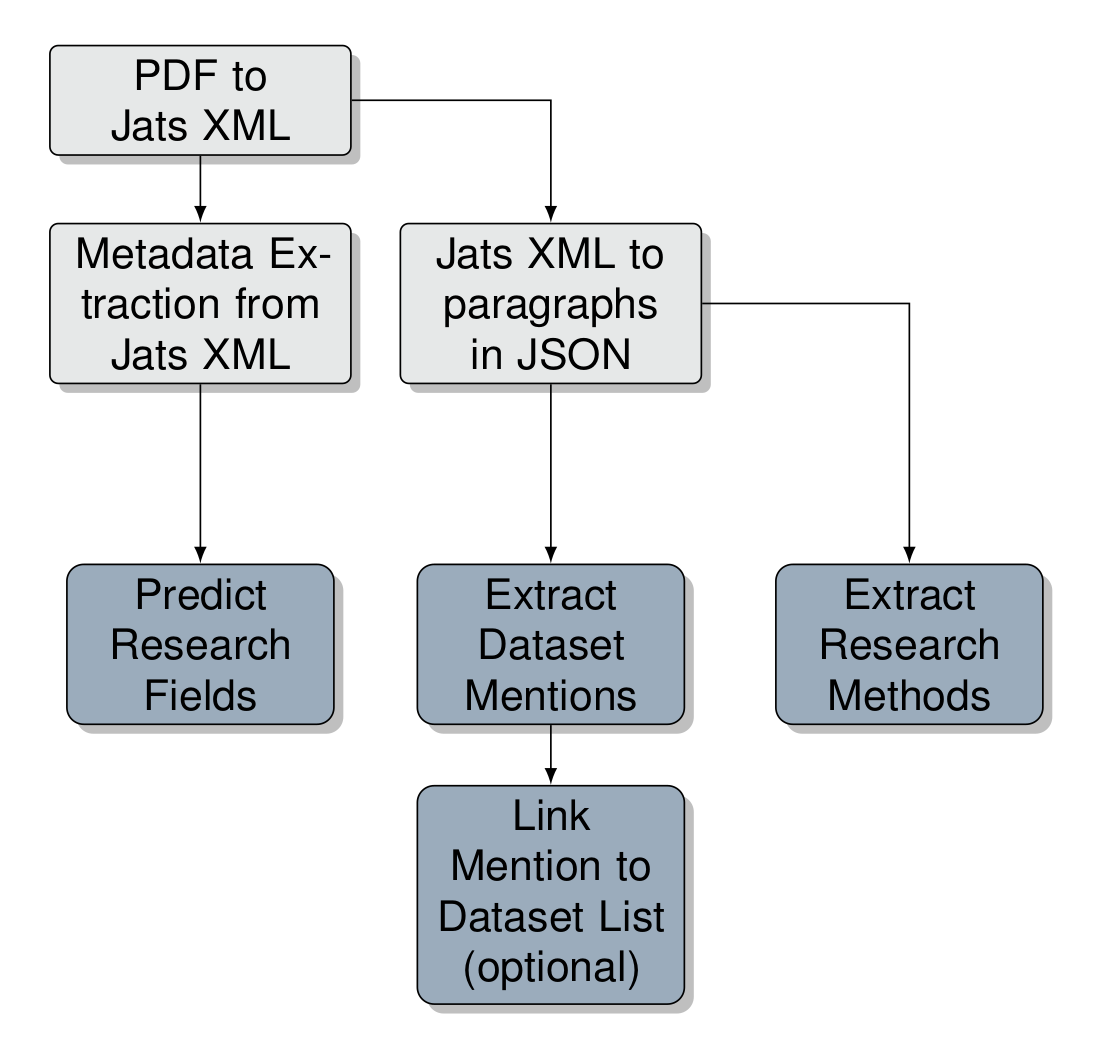
\includegraphics[width=0.47\textwidth]{figures/information-flow.png}
    \caption{Software modules. The figure shows an overview of the individual software modules described in this document and their dependencies. Modules colored in gray represent our pre-processing pipeline, whereas blue-colored modules represent the three main tasks of the RCC.}
    \label{figure:pipeline}
\end{figure}

\subsubsection{First Phase Feedback}
After the first phase, each team received feedback from the organizers of the RCC.
The feedback is twofold and consists of a quantitative and qualitative evaluation. Unfortunately, our team did not perform very well regarding precision and recall. In contrast to this, our approach has been found convincing regarding the quality of results. The qualitative feedback result from a random sample of ten documents that are given to four judges.
Judges are then asked to manually extract dataset mentions and calculate the overlap between their dataset extractions and the output of our algorithm.
Other factors that judges took into consideration are specificity, uniqueness and multiple occurrences of dataset mentions.
As for the extraction of research methods and fields no ground truth has been provided, these tasks were evaluated against the judges' expert knowledge.
Similarly to the extraction of dataset mentions, specificity and uniqueness have been considered for these two tasks.
The feedback our team received acknowledged the fact that no ground truth has been provided and our efforts regarding the extraction of research methods and fields.
%Feedback by RCC
%Section~\ref{} gives detailed overview of data provided by the RCC and additional data sources used in our approach. :o .
